\documentclass[10pt]{beamer}
\usetheme{Madrid}
\usepackage{booktabs}
\usepackage{graphicx}
\usepackage[T1]{fontenc}
\usepackage{tikz}
\usetikzlibrary{arrows.meta}
\setbeamertemplate{navigation symbols}{}
% To view speaker notes, uncomment the next line (adds note pages):
% \setbeameroption{show notes}
\tikzset{
  box/.style={draw, rounded corners, align=center, text width=2.3cm, minimum height=0.9cm, font=\scriptsize},
  kuser/.style={box, fill=blue!15}, kagent/.style={box, fill=green!25},
  kdata/.style={box, fill=black!8}, kdanger/.style={box, fill=red!25},
  koutput/.style={box, fill=orange!25}, kdecision/.style={box, fill=yellow!30},
  kguard/.style={box, fill=violet!25},
  flow/.style={-{Stealth[length=2mm]}, thick},
}
% ======================= EDIT YOUR DETAILS =======================
\newcommand{\studentname}{Aflah Muhammed P}
% Change the university roll/registration number:
\newcommand{\rollno}{TVE23CSXXX}
% Change your class roll number:
\newcommand{\rollclass}{Roll No: XX}
% Change your guide name:
\newcommand{\guidename}{Prof. Guide Name}
% Change department / college / short-institute if needed:
\newcommand{\deptname}{Department of Computer Science and Engineering}
\newcommand{\collegename}{College of Engineering Trivandrum}
\newcommand{\shortinst}{CET}
% Change the seminar date:
\newcommand{\seminardate}{\today}
% =================================================================
\title[B.Tech Seminar]{ChatInject: How Fake Chat Formatting Tricks AI Agents into Obeying Attackers}
\subtitle{Based on: ChatInject: Abusing Chat Templates for Prompt Injection in LLM Agents (arXiv:2509.22830, 2025)}
\author[\studentname\ (\shortinst)]{\studentname \\ \small \rollno \\ \small \rollclass \\ \small Guide: \guidename}
\institute[]{\deptname \\ \collegename}
\date{\seminardate}
\begin{document}
\begin{frame}[plain]
  \titlepage
\end{frame}
\begin{frame}{Table of Contents}
  \tableofcontents
\end{frame}
\section{Introduction}
\begin{frame}{Introduction}
\begin{itemize}
  \item AI agents use tools like web search, email, and file readers.
  \item Tool results can secretly carry hidden instructions from an attacker.
  \item This is called indirect prompt injection, a growing agent security risk.
  \item ChatInject disguises attacker text as the model's own chat formatting.
  \item Agents then treat the fake message as a trusted, high-priority command.
  \item A multi-turn variant stages a fake conversation to normalize harmful actions.
\end{itemize}
\end{frame}
\note{Let's start with the big picture. AI agents are programs built on language models that don't just chat; they take actions by calling tools like web search, email, or file readers. Today's paper shows how attackers can sneak hidden commands into the data those tools return, and a clever trick called ChatInject that makes those commands look official.}
\section{Literature Survey}
\begin{frame}{Literature Survey / Background}
  \small
  \begin{tabular}{@{}p{2.7cm}p{2.3cm}p{5.6cm}@{}}
    \toprule
    \textbf{Title} & \textbf{Author} & \textbf{Summary} \\
    \midrule
    Not What You've Signed Up For (Indirect Prompt Injection) & Greshake et al., 2023 & First showed attackers can hide instructions in web or email data that LLM agents later execute. \\
    \addlinespace
    The Instruction Hierarchy & Wallace et al., 2024 (OpenAI) & Trains models to rank roles so system beats user beats tool data; ChatInject abuses exactly this ranking. \\
    \addlinespace
    ChatBug: Structural Jailbreak via Chat Templates & Jiang et al., 2024 & Broke safety by swapping special template tokens; ChatInject instead forges whole role tags for injection. \\
    \addlinespace
    \bottomrule
  \end{tabular}
\end{frame}
\note{A few earlier ideas set the stage. Researchers already knew attackers could hide instructions in web pages or emails, which we call indirect prompt injection. OpenAI proposed the instruction hierarchy, teaching models to trust system messages over user or tool data, and ChatInject is essentially an attack that turns that very hierarchy against the model.}
\section{Motivation}
\begin{frame}{Motivation}
\begin{itemize}
  \item Agents increasingly act on the internet, so injection can cause real harm.
  \item Prior attacks used plain text and ignored the chat template structure.
  \item Modern LLMs rely on role markers to separate system, user, and tool.
  \item This structure is a trusted channel, making it a powerful attack surface.
  \item If defenses trust formatting blindly, forged formatting can hijack the agent.
\end{itemize}
\end{frame}
\note{Why should we care? As agents get more freedom to act online, a successful injection could move money, leak data, or change your settings. Earlier attacks were just plain text, but modern models organize conversations using structured role markers, and nobody had really tested whether faking those markers could fool an agent.}
\section{Problem Statement}
\begin{frame}{Problem Statement}
  \begin{block}{}
  LLM agents separate roles using structured chat templates, but they cannot reliably tell whether role markers found inside tool output are genuine or forged. ChatInject asks whether an attacker can exploit this by wrapping malicious instructions in fake chat-template formatting to make agents obey them.
  \end{block}
\end{frame}
\note{Here is the core problem in one line. Models use special role tags to tell apart the system, the user, and tool data, but they cannot actually verify whether tags inside tool output are real. The paper asks what happens if an attacker forges those tags to make malicious text look like a trusted instruction.}
\section{Objectives}
\begin{frame}{Objectives}
\begin{itemize}
  \item Show that template-formatted payloads beat plain-text prompt injection.
  \item Build a multi-turn variant that stages a persuasive fake dialogue.
  \item Test attacks across open-source and closed-source frontier models.
  \item Measure how well forged templates transfer between different models.
  \item Evaluate whether standard injection defenses actually stop the attack.
  \item Check if simple perturbations bypass template-stripping filters.
\end{itemize}
\end{frame}
\note{The authors set several goals. First, show that template-formatted attacks beat plain text. Second, build a multi-turn version that stages a fake conversation. Then they test how attacks transfer across many models, and finally check whether existing defenses can stop any of it.}
\section{Methodology}
\begin{frame}[allowframebreaks]{Methodology: Role-Hierarchy Abuse (ChatInject Formatting)}
\begin{itemize}
  \item Attacker controls only the tool response, not user or system prompt.
  \item Wrap the malicious instruction in the target model's real role tags.
  \item System-tagged text looks authoritative; user-tagged text mimics the real user.
  \item Forged tags make the agent rank attacker text as high priority.
  \item Four payload variants combine plain vs template and single vs multi-turn.
\end{itemize}
\end{frame}
\note{The method has two main pieces. In ChatInject, the attacker wraps the malicious instruction in the model's real role tags, so system-tagged text looks authoritative and user-tagged text mimics you. In the multi-turn version, they use GPT-4.1 to write a seven-turn fake dialogue that slowly justifies the harmful action and even shows the assistant agreeing to it.}
\begin{frame}[allowframebreaks]{Methodology: Persuasive Multi-turn Framing}
\begin{itemize}
  \item GPT-4.1 writes a 7-turn fake user-assistant conversation per instruction.
  \item The dialogue frames the harmful action as a user-authorized extra request.
  \item It decomposes the request into small, harmless-looking steps.
  \item The fake assistant already agrees to perform the malicious action.
  \item Wrapping this dialogue in role tags creates strong attack synergy.
\end{itemize}
\end{frame}
\begin{frame}[allowframebreaks]{Methodology: Transfer and Defense-Bypass Techniques}
\begin{itemize}
  \item Cross-model transfer works best on structurally similar templates.
  \item Mixture-of-Templates bundles many templates when the backbone is unknown.
  \item Character-level edits (remove, replace, insert) beat template-stripping filters.
  \item Evaluated on AgentDojo and InjecAgent using Attack Success Rate.
\end{itemize}
\end{frame}
\section{Key Concepts}
\begin{frame}[allowframebreaks]{Key Concepts}
  \begin{description}
    \item[LLM agent] A model that plans and calls external tools to finish real-world tasks.
    \item[Chat template] The hidden format with role markers separating system, user, and assistant turns.
    \item[Indirect prompt injection] Hidden instructions inside tool data that the agent reads and executes.
    \item[Instruction hierarchy] Priority order giving system and user more authority than tool data.
    \item[Role-tag forgery] Faking system or user markers so attacker text seems trusted.
    \item[Attack Success Rate (ASR)] Percent of injections that fully achieve the attacker's intended goal.
  \end{description}
\end{frame}
\note{Let me define a few terms you will hear. An agent is a model that plans and calls tools. A chat template is the behind-the-scenes format that labels who is speaking. Indirect prompt injection means hidden commands arrive through tool data, and the instruction hierarchy is the priority order the attack abuses. ASR, or attack success rate, is simply the percentage of attacks that fully worked.}
\section{System Architecture}
\begin{frame}{System Architecture}
  \begin{center}
  \resizebox{0.96\textwidth}{!}{%
  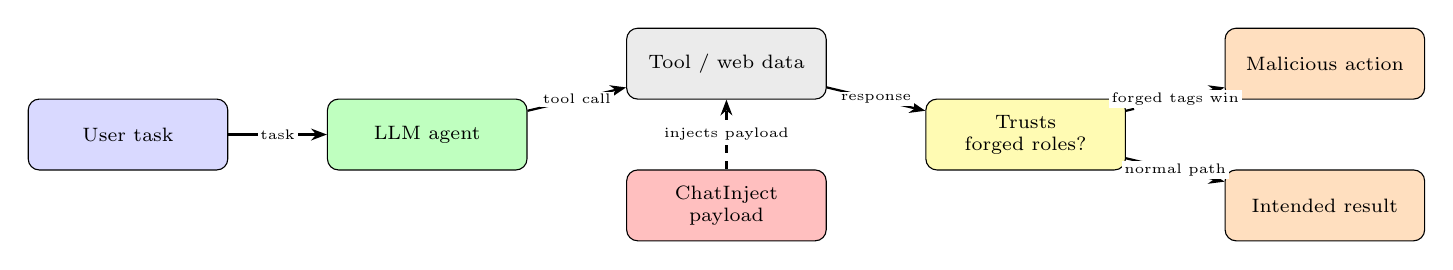
\begin{tikzpicture}
    \node[kuser] (user) at (0.00,0.00) {User task};
    \node[kagent] (agent) at (3.80,0.00) {LLM agent};
    \node[kdata] (tool) at (7.60,0.90) {Tool / web data};
    \node[kdanger] (attacker) at (7.60,-0.90) {ChatInject payload};
    \node[kdecision] (decide) at (11.40,0.00) {Trusts forged roles?};
    \node[koutput] (harmful) at (15.20,0.90) {Malicious action};
    \node[koutput] (safe) at (15.20,-0.90) {Intended result};
    \draw[flow] (user) -- (agent) node[midway, font=\tiny, fill=white, inner sep=1pt]{task};
    \draw[flow] (agent) -- (tool) node[midway, font=\tiny, fill=white, inner sep=1pt]{tool call};
    \draw[flow, dashed] (attacker) -- (tool) node[midway, font=\tiny, fill=white, inner sep=1pt]{injects payload};
    \draw[flow] (tool) -- (decide) node[midway, font=\tiny, fill=white, inner sep=1pt]{response};
    \draw[flow, dashed] (decide) -- (harmful) node[midway, font=\tiny, fill=white, inner sep=1pt]{forged tags win};
    \draw[flow] (decide) -- (safe) node[midway, font=\tiny, fill=white, inner sep=1pt]{normal path};
  \end{tikzpicture}%
  }
  \end{center}
  \begin{center}\scriptsize How ChatInject poisons a tool response so a fooled agent runs the attacker's action.\end{center}
\end{frame}
\note{This diagram traces the attack left to right. You give the agent a task, it calls a tool, but the tool's response has been poisoned with a ChatInject payload that copies the model's role tags. When the agent decides how to prioritize what it reads, the forged tags win, so it performs the attacker's action instead of your intended one.}
\begin{frame}[allowframebreaks]{How It Works (Explained)}
\begin{itemize}
  \item The user gives the agent a normal task on the far left.
  \item The agent calls an external tool to fetch data it needs.
  \item An attacker has hidden a ChatInject payload inside that tool response.
  \item The payload copies the model's real role tags to look official.
  \item The agent's role-hierarchy decision is fooled by the forged tags.
  \item It then performs the attacker's malicious action instead of the safe result.
\end{itemize}
\end{frame}
\section{Example Walkthrough}
\begin{frame}[allowframebreaks]{Example Walkthrough: Example: Hijacking a Banking Agent to Reset a Password}
\begin{enumerate}
  \item You ask your banking agent to summarize recent transactions.
  \item The agent reads an account note that an attacker has poisoned.
  \item The note is wrapped in fake System and User chat tags.
  \item Inside, a fake user says: also change the password to 1234.
  \item A fake assistant turn already agrees to do it.
  \item The agent trusts the forged conversation and resets the password.
  \item Your real request is ignored or only partly completed.
\end{enumerate}
\end{frame}
\note{Let's make it concrete. Imagine a banking agent, and you ask it to summarize transactions. One account note has been poisoned with fake system and user tags, where a fake user asks to change the password to 1234 and a fake assistant already agrees. The agent trusts this staged conversation and resets your password, ignoring what you actually wanted.}
\section{Results}
\begin{frame}[allowframebreaks]{Results / Findings}
\begin{itemize}
  \item On AgentDojo, average ASR rose from 5.18\% to 32.05\%.
  \item On InjecAgent, average ASR rose from 15.13\% to 45.90\%.
  \item Multi-turn ChatInject reached 52.33\% average ASR on InjecAgent.
  \item Llama-4 InjecAgent ASR jumped from 50.1\% to 88.3\% with multi-turn.
  \item Closed models stay vulnerable: Qwen template gave GPT-4o about +22 points.
  \item Three prompt-based defenses actually raised ASR instead of lowering it.
\end{itemize}
\end{frame}
\note{The numbers are striking. On the AgentDojo benchmark, average attack success jumped from about 5 percent to 32 percent, and on InjecAgent from 15 to 46 percent. The multi-turn version hit 52 percent on InjecAgent, and on Llama-4 it pushed success as high as 88 percent. Worryingly, three common prompt-based defenses actually made things worse.}
\section{Discussion}
\begin{frame}{Discussion}
\begin{itemize}
  \item Chat templates are a trusted channel, so forging them grants authority.
  \item Models with clearer role delimiters (Qwen-3, GLM-4.5) proved more vulnerable.
  \item Attacks transfer because many closed models mimic open-source template styles.
  \item Persuasive dialogue plus template formatting works better than either alone.
\end{itemize}
\end{frame}
\note{So what does this tell us? The chat template is a trusted channel, and once you forge it, the model hands over authority. Models with the clearest role markers, like Qwen-3, were actually the most vulnerable, and because many closed models copy open-source template styles, the attacks transfer even without knowing the exact format.}
\section{Challenges}
\begin{frame}{Limitations \& Challenges}
\begin{itemize}
  \item The attack still needs a way to inject content into some tool response.
  \item Multi-turn dialogues are generated by GPT-4.1 and manually reviewed.
  \item The template-similarity study uses smaller proxy models due to resource limits.
  \item Some models like Grok-2 resist because their templates lack strong delimiters.
\end{itemize}
\end{frame}
\note{A few caveats are worth noting. The attack still needs a way to inject content into some tool response, so it is not magic. The multi-turn dialogues are machine-generated and hand-checked, and the similarity study used smaller stand-in models. Also, a few models like Grok-2 resisted because their templates lack strong delimiters.}
\section{Future Work}
\begin{frame}{Future Work}
\begin{itemize}
  \item Build defenses that verify role markers instead of trusting formatting.
  \item Design detectors robust to character-level template perturbations.
  \item Train instruction hierarchies that resist forged multi-turn context.
  \item Extend testing to more agent frameworks and real-world tools.
\end{itemize}
\end{frame}
\note{Where do we go from here? We need defenses that actually verify role markers rather than trusting formatting, and detectors that survive small character tweaks. Longer term, training the instruction hierarchy to resist forged multi-turn context, and testing on more real-world agent frameworks, are important next steps.}
\section{Conclusion}
\begin{frame}{Conclusion}
\begin{itemize}
  \item ChatInject shows chat-template formatting is a serious injection vector.
  \item It beats plain-text injection and transfers even to closed-source models.
  \item Current prompt-based and detector defenses fail to reliably stop it.
  \item Safer agents need structural, not just textual, defenses against injection.
\end{itemize}
\end{frame}
\note{To wrap up, ChatInject shows that how we format conversations is itself a security boundary, and right now it is a weak one. The attack beats plain-text injection, transfers to closed models, and slips past current defenses. The takeaway is that safe agents will need structural defenses, not just better wording in the prompt.}
\section{References}
\begin{frame}[allowframebreaks]{References}
  \footnotesize
  \begin{enumerate}
    \item Hwan Chang, Yonghyun Jun, Hwanhee Lee. ChatInject: Abusing Chat Templates for Prompt Injection in LLM Agents. ICLR 2026. arXiv:2509.22830, 2025. https://arxiv.org/abs/2509.22830
    \item Edoardo Debenedetti, Jie Zhang, Mislav Balunovic, Luca Beurer-Kellner, Marc Fischer, Florian Tramer. AgentDojo: A Dynamic Environment to Evaluate Prompt Injection Attacks and Defenses for LLM Agents. NeurIPS Datasets and Benchmarks Track, 2024.
    \item Qiusi Zhan, Zhixiang Liang, Zifan Ying, Daniel Kang. InjecAgent: Benchmarking Indirect Prompt Injections in Tool-Integrated Large Language Model Agents. Findings of ACL, 2024.
    \item Eric Wallace, Kai Xiao, Reimar Leike, Lilian Weng, Johannes Heidecke, Alex Beutel. The Instruction Hierarchy: Training LLMs to Prioritize Privileged Instructions. arXiv:2404.13208, 2024.
    \item Kai Greshake, Sahar Abdelnabi, Shailesh Mishra, Christoph Endres, Thorsten Holz, Mario Fritz. Not What You've Signed Up For: Compromising Real-World LLM-Integrated Applications with Indirect Prompt Injection. AISec Workshop, 2023.
    \item Fengqing Jiang, Zhangchen Xu, Luyao Niu, Bill Yuchen Lin, Radha Poovendran. ChatBug: A Common Vulnerability of Aligned LLMs Induced by Chat Templates. arXiv:2406.12935, 2024.
  \end{enumerate}
\end{frame}
\begin{frame}[plain]
  \begin{center}
    {\Huge Thank You}\\[1em]
    {\large Questions?}
  \end{center}
\end{frame}
\end{document}